\documentclass{article}

\usepackage[utf8]{inputenc}
\usepackage[T1]{fontenc}
\usepackage[brazilian]{babel}

\usepackage{microtype}

\usepackage{xcolor}
\usepackage{graphicx}
\usepackage{pgfplots}
\pgfplotsset{compat=1.18}
\usetikzlibrary{fit}

\usepackage{array}
\usepackage{booktabs}
\usepackage{multirow}
\usepackage{tabularx}
\usepackage{longtable}

\usepackage{url}
\usepackage{listings}

\usepackage{relsize}
\newcommand{\cpp}{C\nolinebreak\hspace{-.05em}\raisebox{.4ex}{\relsize{-3}{\textbf{+}}}\nolinebreak\hspace{-.10em}\raisebox{.4ex}{\relsize{-3}{\textbf{+}}}}
\newcommand{\ccpp}{C\slash\cpp}

\lstdefinestyle{macrocode}{
    backgroundcolor  = \color{white},
    rulesepcolor     = \color{darkgray},
    commentstyle     = \color{gray},
    keywordstyle     = \color{blue}\bfseries,
    stringstyle      = \color{purple},
    basicstyle       = \ttfamily\footnotesize,
    showspaces       = false,
    showstringspaces = false,
    numbers          = left,
    tabsize          = 1,
    numberstyle      = \scriptsize,
    frame            = shadowbox,
    breaklines       = true,
    captionpos       = b,
}

\renewcommand{\lstlistingname}{Código}
\renewcommand{\lstlistlistingname}{Lista de Códigos}

\usepackage{todonotes}
\newcommand{\scene}[2]{\todo[size=\tiny,color=blue!10]{#1 (#2)}}

\usepackage{caption}
\usepackage{subcaption}

\newcommand{\ark}{\textsc{ArKanjo}}
\newcommand{\vnova}{\texttt{v0.7.0-rc}}

\usetikzlibrary{positioning,arrows.meta}

\definecolor{v070}{HTML}{2C6478}

\newcolumntype{P}[1]{>{\raggedright\arraybackslash}p{#1}}

\usepackage[hidelinks]{hyperref}

\title{Estudo e mitigação de duplicações em projetos FLOSS utilizando a ferramenta \ark}

\author{Guilherme Ivo Bozi\thanks{O presente trabalho foi realizado com apoio da Fundação de Amparo à Pesquisa do Estado de São Paulo (FAPESP), Brasil. Processo nº 2025/22416-1.}\\
\small{MAC0214 -- Atividade Curricular em Cultura e Extensão (2026)} \\
\small{Instituto de Matemática, Estatística e Ciência da Computação (IME)} \\
\small{Universidade de São Paulo (USP)}}

\date{Segundo semestre de 2026}

\begin{document}

\renewcommand{\thefootnote}{\fnsymbol{footnote}}
\setcounter{footnote}{1}

\maketitle

\renewcommand{\thefootnote}{\arabic{footnote}}
\setcounter{footnote}{0}

\begin{abstract}
O \ark{} é uma ferramenta de detecção de duplicações de código em nível de função desenvolvida pelo nosso grupo de pesquisa. Este trabalho aplicou a ferramenta a sete projetos de software livre (\textsc{NGINX}, \textsc{Git}, \textsc{Apache HTTP Server}, \textsc{CPython}, kernel Linux, \textsc{LLVM} e \textsc{GIMP}) com dois objetivos: encontrar problemas da própria ferramenta em códigos reais e usar os resultados para identificar oportunidades de refatoração nesses projetos. Por exemplo, as execuções revelaram um \emph{stack overflow} ao processar um arquivo de teste do \textsc{LLVM} com 16.384 níveis de chaves aninhadas e colisões no cache entre funções com mesmos nomes no mesmo arquivo, além de necessidades específicas de uso em bases grandes. Esses achados foram registrados como \textit{issues} e relatados na discussão de execuções em projetos reais. Em paralelo, foram desenvolvidas contribuições à ferramenta (\texttt{v0.5.2} a \vnova{}), entre elas uma terminação antecipada no cálculo de similaridade entre árvores sintáticas, identificada a partir de perfis de execução, e uma refatoração no armazenamento dos resultados. Para apoiar a análise, foram construídas duas visualizações da duplicação no kernel Linux, uma com \textit{hierarchical edge bundling} (HEB) e outra com um \textit{treemap} ponderado por similaridade. Entre as versões \texttt{v0.5.1} e \vnova{}, a taxa de sucesso subiu de 71\% para 86\% dos repositórios e o tempo de análise do kernel Linux caiu de cerca de 4 dias para cerca de 17 min; a aceleração cresce com o tamanho do projeto, de $\times$22 no \textsc{NGINX} a $\times$342 no Linux. Uma análise preliminar das duplicações encontradas apontou possíveis contribuições aos projetos analisados.
\end{abstract}

\scene{Scene 0}{0:00--0:20}

\clearpage

\section{Introdução}

\scene{Scene 1}{0:20--1:30}

Desenvolvedores frequentemente reutilizam código copiando, colando e adaptando trechos existentes. A duplicação resultante é um \emph{code smell} conhecido~\cite{fowler2018refactoring} e uma forma de \emph{dívida técnica}~\cite{kruchten2012debt,seaman2011measuring}: qualquer mudança em uma cópia, como a correção de um defeito, precisa ser propagada para as demais, e alterações inconsistentes em clones são uma fonte documentada de falhas~\cite{juergens2009clones}. Mesmo em projetos com revisão de código rigorosa, como o kernel Linux, duplicações de funções inteiras e até de diretórios podem continuar presentes~\cite{kumar2016bigclones}.

O \ark{}~\cite{arcanjo2025debconf,arcanjo2025dissertacao} é uma ferramenta desenvolvida pelo nosso grupo de pesquisa para detectar duplicações em nível de função. Ela identifica as funções presentes em cada arquivo-fonte, guarda essas informações em cache e compara as funções entre si com base em um nível de similaridade definido pelo usuário, utilizando métodos estabelecidos. A ferramenta foi usada no projeto de iniciação científica que dá origem a esta atividade, voltado a duplicações no kernel Linux, e no estudo do grupo sobre como a comunidade do kernel recebe \emph{patches} de deduplicação~\cite{duplicationdebt2026}. Esse estudo analisou 101 contribuições e observou, entre outros pontos, que os mantenedores aceitam com mais facilidade refatorações que reutilizam abstrações já existentes do que as que criam novas.

Testes controlados não cobrem toda a variedade de código encontrada em projetos reais. Arquivos com milhares de níveis de aninhamento, funções com mesmos nomes separadas por diretivas de pré-processador, macros que se parecem com chamadas de função e bases com milhões de pares de clones expõem falhas de análise, falsos positivos, falsos negativos, \textit{crashes} e problemas de desempenho.

\section{Objetivos}

\scene{Scene 2}{1:30--2:15}

O objetivo geral foi avaliar o \ark{} em condições próximas do uso cotidiano, contribuir para o seu aprimoramento e usar os resultados para identificar oportunidades de refatoração nos projetos analisados~\cite{arkanjodiscussions}. Os objetivos específicos foram:

\begingroup
\renewcommand{\labelenumi}{(\alph{enumi})}
\begin{enumerate}
  \item executar o \ark{} em projetos FLOSS e identificar duplicações em nível de função;
  \item investigar e documentar falsos positivos, falsos negativos, \textit{crashes} e falhas de \emph{parsing};
  \item abrir \textit{issues} com os problemas identificados e, quando possível, desenvolver e testar correções na ferramenta;
  \item gerar e analisar visualizações e relatórios de duplicação para apoiar a seleção de casos de refatoração;
  \item propor e, quando possível, submeter \textit{patches} de refatoração aos projetos analisados;
  \item caso sejam submetidos \textit{patches} de refatoração, acompanhar a revisão das contribuições e registrar a interação com as comunidades.
\end{enumerate}
\endgroup

\section{Materiais e Métodos}

\scene{Scene 3}{2:15--4:00}

\subsection{Projetos analisados}

Na seleção foram escolhidos sete projetos escritos majoritariamente em \ccpp{} e Python, com tamanhos e estilos de organização diferentes (Tabela~\ref{tab:projetos}). Todos os repositórios foram clonados com histórico completo.

\begin{table}[ht!]
\centering
\caption{Projetos analisados.}
\label{tab:projetos}
\begin{tabular}{ll}
\toprule
\textbf{Projeto} & \textbf{HEAD analisado} \\
\midrule
\textsc{NGINX}~\cite{nginx} & \texttt{ef0aa967dce9} \\
\textsc{Git}~\cite{git} & \texttt{d38352cd43ab} \\
\textsc{Apache HTTP Server} (httpd)~\cite{apache_httpd} & \texttt{54730cc72552} \\
\textsc{CPython}~\cite{cpython} & \texttt{9193375382fb} \\
Kernel Linux~\cite{linux_kernel} & \texttt{9b87fdc9af2f} \\
\textsc{LLVM} (llvm-project)~\cite{llvm} & \texttt{1c0fc1d0d8ae} \\
\textsc{GIMP}~\cite{gimp} &  \texttt{62a299d45b81} \\
\bottomrule
\end{tabular}
\end{table}

\subsection{A ferramenta \ark}

O \ark{} é escrito em \cpp{} e tem dois estágios (Figura~\ref{fig:arquitetura}). O \emph{Preprocessor} roda uma vez por base de código: o \emph{Function Parser} usa o Tree-sitter~\cite{treesitter} para isolar cada função em três arquivos (assinatura, corpo e metadados com caminho e linhas de início e fim), e o \emph{Duplication Finder} compara as funções e grava os pares cuja similaridade supera o limiar (\texttt{-S}). O \emph{Query Responder} consulta esse resultado sem reprocessar o código. O \emph{Duplication Finder} oferece métodos diferentes: TF-IDF com similaridade de cosseno, AST linearizada e \emph{embeddings} de código.

\begin{figure}[ht!]
\centering
\begin{tikzpicture}[
    box/.style={draw, rounded corners=2pt, minimum height=0.9cm,
                minimum width=3.4cm, align=center, font=\small},
    >={Stealth}]
  \node[box] (in) {Código do\\ projeto};
  \node[box, fill=blue!15, right=0.3cm of in, minimum width=3.9cm] (parser) {Function Parser\\\footnotesize Tree-sitter};
  \node[box, fill=orange!25, right=0.3cm of parser, minimum width=3.9cm] (finder) {Duplication Finder\\\footnotesize TF-IDF / AST / \emph{embeddings}};
  \node[box, below=0.3cm of parser, minimum width=3.9cm] (funcs) {Funções extraídas\\\footnotesize assinatura, corpo, metadados};
  \node[box, below=0.3cm of finder, minimum width=3.9cm] (db) {Base de duplicações\\\footnotesize pares e similaridades};
  \node[box, fill=green!20, below=0.3cm of db, minimum width=3.9cm] (query) {Query Responder\\\footnotesize consultas e análises};
  \draw[->] (in) -- (parser);
  \draw[->] (parser) -- (funcs);
  \draw[->] (funcs) -- (finder);
  \draw[->] (finder) -- (db);
  \draw[->] (db) -- (query);
  \node[draw, dashed, inner sep=2pt, fit=(parser)(finder)(funcs)(db),
        label={[font=\footnotesize]above:Preprocessor (\texttt{arkanjo preprocessor build})}] {};
\end{tikzpicture}
\caption{Arquitetura do \ark{}.}
\label{fig:arquitetura}
\end{figure}

Todas as execuções deste relatório usaram o método \texttt{ast}. O objetivo central era avaliar a ferramenta completa em projetos reais, e não comparar os métodos de detecção, e o método \texttt{ast} é o que tem menor custo nas bases avaliadas. Os outros métodos podem levar mais tempo e consumir mais memória, o que pesa em bases com milhões de funções, como o kernel Linux e o \textsc{LLVM}. Na avaliação com \emph{benchmarks} feita anteriormente~\cite{bozi2026mac0215}, o método por \emph{embeddings} levou 148~s no BigCloneBench, contra 12~s do método \texttt{ast}, mas obteve o melhor F1 nos clones Type-3 e Type-4. Os outros métodos podem, portanto, encontrar duplicações que o \texttt{ast} não encontra.

Um exemplo de execução do pré-processador na base de código do \textsc{LLVM}, com similaridade de 0,80 e utilizando o método de AST linearizada:

\begin{lstlisting}[style=macrocode,numbers=none,language=bash,morekeywords={arkanjo}]
arkanjo preprocessor build --verbose --minimum-lines 3 \
    -S80.0 --path="llvm-project" --name="llvm-cache" --method ast
\end{lstlisting}

\subsection{Ambiente de execução}

O ambiente seguiu a documentação de preparação da ferramenta~\cite{arkanjomethod}, em uma máquina virtual com a configuração da Tabela~\ref{tab:ambiente}.
\begin{table}[ht!]
\centering
\caption{Configuração da máquina usada nas execuções.}
\label{tab:ambiente}
\begin{tabularx}{1.0\textwidth}{l >{\raggedright\arraybackslash}X}
\toprule
Componente & Configuração \\
\midrule
Processador     & Intel Xeon (Sapphire Rapids), 16 vCPUs, 1 \emph{thread} por núcleo \\
Memória         & 62 GiB \\
Virtualização   & KVM (virtualização completa) \\
Sistema         & Debian GNU/Linux 13.8 (trixie) \\
Compilador      & GCC (g++) 14.2.0 (Debian 14.2.0-19) \\
\bottomrule
\end{tabularx}
\end{table}

\subsection{Execuções e métricas}

Foram feitas quatro rodadas sobre os sete repositórios, com a versão estável \texttt{v0.5.1} e com a versão \vnova{}. Esta última ainda não foi lançada oficialmente: é uma versão candidata em fase de testes, compilada a partir da \textit{merge request} \verb|!85|\footnote{\url{https://gitlab.com/ccsl-usp/codev/arkanjo-tool/-/merge_requests/85}} do repositório da ferramenta.

\begin{itemize}
  \item \texttt{v0.5.1} com similaridade 1,00 (rodada inicial, agosto);
  \item \texttt{v0.5.1} com similaridade 0,80;
  \item \vnova{} com similaridade 1,00;
  \item \vnova{} com similaridade 0,80.
\end{itemize}

Para cada rodada foram registrados o \textit{status} por repositório (sucesso/falha), o tempo de execução, o tempo até a falha e os dados gerados pelo \ark{} na base de dados. Esses dados são analisados na Tabela~\ref{tab:execucoes} e nas Figuras~\ref{fig:sucesso}, \ref{fig:tempos} e~\ref{fig:speedup}.

\subsection{Investigação de falhas da ferramenta}

As falhas foram reproduzidas isoladamente, executando a ferramenta só sobre o diretório ou arquivo suspeito. \emph{Crashes} foram investigados com o \textsc{GDB}, coletando o \emph{backtrace} completo de todas as \textit{threads}. Resultados suspeitos, como funções ausentes ou pares inesperados, foram conferidos abrindo os trechos correspondentes no código-fonte. Cada problema confirmado foi registrado como \textit{issue} no repositório da ferramenta, com projeto, \textit{commit}, versão do \ark{} e passos de reprodução.

\subsection{Análise de desempenho}

As melhorias de desempenho foram guiadas por perfis de execução coletados com o \texttt{perf}~\cite{perf}, a ferramenta de \emph{profiling} do Linux baseada em contadores de desempenho. A ferramenta foi executada sob \texttt{perf record} em repositórios representativos, e os perfis gerados foram inspecionados com \texttt{perf report} para identificar as funções que concentravam o tempo de execução. Cada alteração foi avaliada repetindo a coleta e comparando os perfis antes e depois da mudança.

\subsection{Desenvolvimento na ferramenta}

As versões seguem o versionamento semântico (SemVer)~\cite{semver}, no formato \texttt{MAJOR.\allowbreak MINOR\allowbreak.PATCH}. Correções que não mudam o comportamento esperado incrementam o \texttt{PATCH} (por exemplo, \texttt{v0.5.2} a \texttt{v0.5.4}); novas funcionalidades incrementam o \texttt{MINOR} (\texttt{v0.6.0}). Enquanto o \texttt{MAJOR} é 0, a ferramenta está em desenvolvimento inicial e um novo \texttt{MINOR} pode trazer mudanças incompatíveis, como a troca do formato de armazenamento prevista para a \texttt{v0.7.0}. Versões ainda em teste recebem um sufixo de pré-lançamento, como em \vnova{}, que indica que a versão é anterior à \texttt{v0.7.0} definitiva.

\subsection{Visualizações}
\label{sec:metviz}

Para localizar a duplicação em bases grandes foram construídas duas visualizações a partir da saída do \ark{}.

\paragraph{\textit{Hierarchical Edge Bundling} (HEB).} Os arquivos são dispostos em um círculo, agrupados pela hierarquia de diretórios, e cada par de arquivos com funções duplicadas é ligado por uma aresta. As arestas são curvadas ao longo da hierarquia e se agrupam em feixes, técnica proposta por Holten~\cite{holten2006heb}. A implementação partiu do exemplo de Bostock~\cite{bostock_heb}, com rótulos de hierarquia em anéis externos inspirados no \emph{Well-formed Eigenfactor}~\cite{stefaner2009eigenfactor}. A renderização em SVG do D3 foi substituída por uma renderização própria em WebGL2, para desenhar a quantidade de arestas de uma base como o kernel, e a hierarquia foi adaptada para arquivos e relações de duplicação. A visualização pode ser explorada de forma interativa no navegador~\cite{bozi2026duplicationviz} ou exportada como imagem\footnote{\url{https://guilhermeivo.com.br/duplication-viz/}}.

\paragraph{\textit{Treemap} ponderado.} Para um arquivo $p$, seja $N(p)$ o conjunto de arquivos com os quais $p$ tem funções duplicadas e $\mathrm{sim}(p,q)$ a similaridade entre $p$ e $q$. A similaridade média e a similaridade ponderada de $p$ são
\begin{equation}
  \mathrm{AS}(p) = \frac{1}{|N(p)|}\sum_{q \in N(p)} \mathrm{sim}(p,q),
  \qquad
  \mathrm{WS}(p) = \mathrm{LOC}(p)\cdot \mathrm{AS}(p),
\end{equation}
em que $\mathrm{LOC}(p)$ é o número de linhas de código de $p$. No mapa de árvore~\cite{shneiderman1992treemap}, a hierarquia é diretório/subsistema $\rightarrow$ arquivo, a área de cada arquivo é proporcional a $\mathrm{WS}(p)$ e a cor apenas distingue subsistemas. Áreas maiores indicam arquivos maiores, mais parecidos com os arquivos relacionados, ou as duas coisas.

\subsection{Análise preliminar de possíveis contribuições}
\label{sec:triagem}

Para levantar candidatos à refatoração, os pares reportados foram separados por tipo de código (gerado, de terceiros, de teste e de produção) e agrupados em famílias de funções relacionadas. Para as famílias de produção, consultou-se o histórico do git em busca de \textit{commits} que alteraram mais de uma cópia, um indício de que a duplicação já gerou retrabalho. Essa análise foi feita com \textit{scripts}, e por isso os casos que ela aponta são tratados como hipóteses: cada um precisa ser conferido manualmente no código e no histórico antes de virar um \emph{patch}.

\section{Resultados}\label{sec:resultados}

\subsection{Problemas encontrados no \ark}

\scene{Scene 4a}{4:00--4:50}

A Tabela~\ref{tab:bugs} resume os problemas encontrados nas execuções. Os dois mais graves são descritos a seguir.

\paragraph{\emph{Stack overflow} no \textsc{LLVM}.}
Na \texttt{v0.5.1}, a análise do llvm-project terminava com \emph{stack overflow}. A execução no GDB mostrou milhares de chamadas consecutivas a \texttt{TreeSitterParser::\allowbreak collect\_functions()} e identificou o arquivo \texttt{clang/\allowbreak test/\allowbreak Parser/\allowbreak parser\_overflow.c}. Trata-se de um teste do próprio \textsc{LLVM} que, com \texttt{HUGE} definido, cria 16.384 níveis de chaves aninhadas para estressar o \emph{parser}. Como a coleta de funções é recursiva sobre a árvore sintática, a profundidade da pilha acompanha a profundidade do aninhamento. O problema foi registrado como \textit{issue} e relatado na discussão de execuções em projetos reais.

\paragraph{Colisão de \textit{cache} para funções com mesmo nome.}
No kernel Linux, o arquivo que define \texttt{apply\_acpi\_orientation()} tem duas implementações, uma em cada ramo de \texttt{\#ifdef CONFIG\_ACPI}. Como \texttt{FunctionStorage::\allowbreak build\allowbreak\_output\allowbreak\_path()} monta o caminho do \textit{cache} a partir do caminho do arquivo e do nome da função, a segunda implementação lida sobrescreve a primeira, e a função armazenada depende da ordem de leitura. O mesmo ocorre com sobrecarga de funções em \cpp{} e com métodos de mesmo nome em classes diferentes. Isso gera falsos negativos (uma das versões nunca é comparada) e resultados não determinísticos. A refatoração do armazenamento descrita na Seção~\ref{sec:contrib} já centraliza a identificação das funções em um único ponto, mas a identidade usada continua sendo caminho e nome; resolver a \textit{issue} exige acrescentar a ela a assinatura ou a posição da função.

\begin{table}[ht!]
\centering
\caption{Problemas e melhorias do \ark{} identificados a partir das execuções em projetos reais.}
\label{tab:bugs}
\begin{tabularx}{1.0\linewidth}{l >{\raggedright\arraybackslash}X l l}
\toprule
\textbf{Tipo} & \textbf{Descrição} & \textbf{Origem} & \textbf{Situação} \\
\midrule
\emph{Crash} & \emph{Stack overflow} na travessia recursiva da árvore sintática em \texttt{parser\_overflow.c} & \textsc{LLVM} & \textit{issue} \\
Falso negativo & Colisão no \textit{cache} para funções com mesmo nome (\texttt{\#ifdef}, sobrecarga \cpp, métodos de classes diferentes) & Linux & \textit{issue} \\
\emph{Parsing} & Nomes de funções \cpp{} com \texttt{type\_identifier} e \texttt{qualified\_identifier} extraídos incorretamente & \cpp & \texttt{v0.5.2} \\
Usabilidade & Exclusão de arquivos e diretórios (\texttt{-{}-exclude}, \texttt{.gitignore}) & bases grandes & \textit{issue} \\
Reprodutibilidade & Metadados com informação do repositório (\textit{commit}, \textit{branch}, árvore) & todas & \textit{issue} \\
Falha & Análise do \textsc{GIMP} falha em todas as versões & \textsc{GIMP} & em análise \\
\bottomrule
\end{tabularx}
\end{table}

\paragraph{Melhorias de uso.}
Duas \textit{issues} nasceram das dificuldades práticas das execuções: (i) opção repetível \texttt{-{}-exclude} com padrões \emph{glob} e respeito ao \texttt{.gitignore} via \texttt{git\_ignore\_path\_is\_ignored} do libgit2~\cite{libgit2}, para evitar varrer \texttt{build/}, \texttt{third\_party/} e similares; (ii) registro, no \texttt{config.json}, do \textit{commit}, \textit{branch}, estado da árvore de trabalho e \emph{hash} da árvore do repositório analisado, sem falhar quando o diretório não for um repositório git. A segunda permite saber exatamente qual versão de cada projeto gerou um resultado.

\subsection{Contribuições ao \ark}\label{sec:contrib}

\scene{Scene 4b}{4:50--5:25}

Além de registrar problemas, o trabalho incluiu desenvolvimento na própria ferramenta. Entre agosto e novembro foram publicadas cinco versões, de \texttt{v0.5.2} a \texttt{v0.6.1}, e a \vnova{} está em desenvolvimento desde outubro (Figura~\ref{fig:versoes}). A Tabela~\ref{tab:contrib} agrupa as principais mudanças por tema.

\begin{figure}[ht!]
\centering
\begin{tikzpicture}[x=0.1cm]
  \draw[->, gray] (0,0) -- (118,0);
  \foreach \x/\m in {0/ago,31/set,61/out,92/nov}
    {\draw[gray] (\x,0.12) -- (\x,-0.12) node[below, font=\footnotesize, black] {\m};}
  \foreach \x/\t in {3/v0.5.1,27/v0.5.2,71/v0.5.3,97/v0.5.4,100/v0.6.0,103/v0.6.1}
    {\fill[v070] (\x,0) circle (2pt);
     \node[rotate=90, anchor=west, font=\footnotesize\ttfamily] at (\x,0.15) {\t};}
  \fill[orange!35] (69,-0.95) rectangle (114,-0.65);
  \draw[orange!70!black, dashed] (69,-0.95) rectangle (114,-0.65);
  \draw[->, orange!70!black] (114,-0.8) -- (118,-0.8);
  \node[font=\footnotesize, anchor=north] at (91.5,-1.0)
    {\vnova{} em desenvolvimento};
\end{tikzpicture}
\caption{Versões do \ark{} publicadas no período (pontos) e período de
desenvolvimento da \vnova{} (faixa), iniciado em outubro. A \texttt{v0.5.1},
usada como referência nas execuções, é anterior às contribuições deste
trabalho.}
\label{fig:versoes}
\end{figure}

{\setlength{\tabcolsep}{4pt}
\begin{longtable}{P{0.20\linewidth}P{0.55\linewidth}P{0.15\linewidth}}
\caption{Principais contribuições ao \ark{} no período, agrupadas por tema.}
\label{tab:contrib}\\
\toprule
\textbf{Tema} & \textbf{Mudanças} & \textbf{Versão} \\
\midrule
\endfirsthead
\toprule
\textbf{Tema} & \textbf{Mudanças} & \textbf{Versão} \\
\midrule
\endhead
\bottomrule \\
\multicolumn{3}{P{\linewidth}}{\footnotesize \textsuperscript{a} Um traço (---) indica que a contribuição não está associada a uma versão específica.}
\endlastfoot
Desempenho & Terminação antecipada no cálculo de similaridade entre árvores sintáticas: o cálculo para quando a menor distância de uma linha da programação dinâmica ultrapassa o limite permitido pelo limiar, preservando o valor exato dos pares que atingem o limiar. & \texttt{v0.6.0} \\
\emph{Parsing} & Extração de nomes com \texttt{type\_identifier} como alternativa e verificação de nós internos de \texttt{qualified\_identifier}. & \texttt{v0.5.2} \\
Armazenamento & Registro de funções com identificadores de 64 bits (FNV-1a) e detecção de colisões de \emph{hash}; migração do armazenamento das duplicações para um formato binário, com tabelas de \emph{strings}, funções, metadados e similaridades; construção do caminho de saída centralizada em \texttt{FunctionStorage}. & \texttt{v0.7.0-rc} \\
Correções & Criação dos diretórios de saída antes da escrita; validação do \texttt{base-path}; validação da leitura de Similaridade. & \texttt{v0.5.3} a \texttt{v0.6.1} \\
Dependências & libgit2 atualizada de 1.9.1 para 1.9.7 e troca do PCRE (fora de suporte) pelo PCRE2 (dependência do libgit2). & ---\textsuperscript{a} \\
Integração contínua & Migração do GitHub Actions para o GitLab CI, junto com os modelos de issue; \emph{pipeline} dividido em módulos, verificação de formatação com \texttt{clang-format} e regras para evitar execuções desnecessárias. & ---\textsuperscript{a} \\
Interface & Mensagens de erro formatadas; variáveis de ambiente com precedência sobre os valores padrão do CMake; ajuda com descoberta de comandos externos. & \texttt{v0.6.0} \\
Comunidade & Revisão e integração de uma contribuição externa. & ---\textsuperscript{a} \\
\end{longtable}}

\subsection{Desempenho e robustez entre versões}

\scene{Scene 4c}{5:25--6:30}

A Tabela~\ref{tab:execucoes} e a Figura~\ref{fig:sucesso} resumem as rodadas concluídas. A \vnova{} terminou a análise em 6 dos 7 repositórios; a única falha restante é o \textsc{GIMP}, que falhou em todas as versões (na \texttt{v0.5.1}, após 164 s). O \textsc{LLVM}, que falhava na \texttt{v0.5.1}, passou a ser analisado em 28 min 59 s.

\begin{table}[ht!]
\centering
\caption{Resumo das rodadas de execução nos 7 repositórios.}
\label{tab:execucoes}
\begin{tabular}{lcccrr}
\toprule
\textbf{Versão} & \textbf{Similaridade} & \textbf{Sucesso} & \textbf{Taxa} & \textbf{Tempo total} & \textbf{Cache} \\
\midrule
\texttt{v0.5.1} & 1,00 & 5/7 & 71\% & 97 h 49 min & 917,2 MiB \\
\texttt{v0.5.1} & 0,80 & 5/7 & 71\% & 99 h 33 min & 1.228,8 MiB \\
\vnova{} & 1,00 & 6/7 & 86\% & 46 min 50 s & 809,0 MiB \\
\vnova{} & 0,80 & 6/7 & 86\% & 8 h 39 min  & 941,4 MiB \\
\bottomrule
\end{tabular}
\end{table}

\begin{figure}[ht!]
\centering
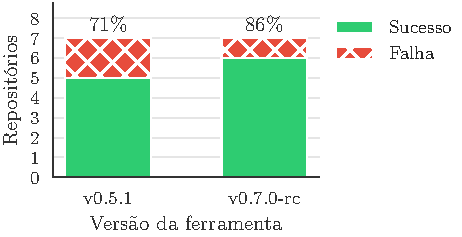
\includegraphics[width=0.7\linewidth]{figures/outcomes_by_version.pdf}
\caption{Sucessos e falhas por versão, similaridade 1,00 (71\% contra 86\%).}
\label{fig:sucesso}
\end{figure}

A Figura~\ref{fig:tempos} compara o tempo por repositório. Nos cinco repositórios analisados com sucesso nas duas versões, a soma dos tempos caiu de cerca de 97,8 h para cerca de 18 min. A maior diferença está no kernel Linux: 347.919 s (cerca de 4 dias) na \texttt{v0.5.1} contra 1.017 s (16 min 57 s) na \vnova{}. No \textsc{CPython} o tempo caiu de cerca de 1 h para 39 s; no \textsc{Git}, de 5 min 07 s para 4,9 s; no httpd, de 3 min 18 s para 6,8 s; e no \textsc{NGINX}, de 53 s para 2,4 s.

\begin{figure}[ht!]
\centering
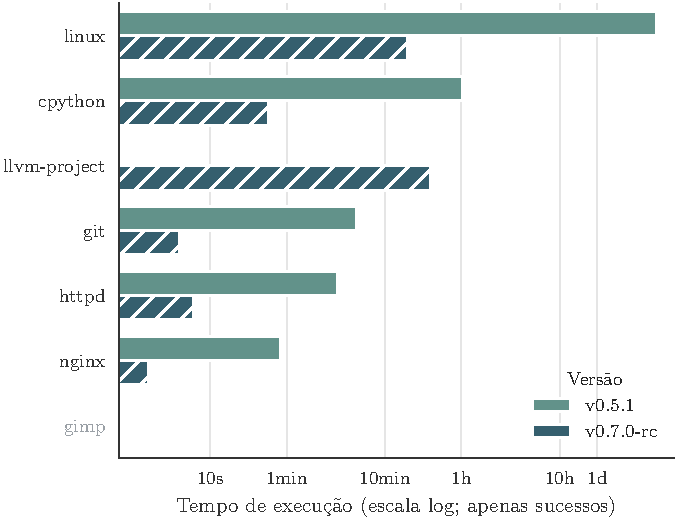
\includegraphics[width=\linewidth]{figures/time_by_repository.pdf}
\caption{Tempo de execução por repositório e versão, similaridade 1,00. O
\textsc{LLVM} falhou na \texttt{v0.5.1} e o \textsc{GIMP} falhou nas duas versões.}
\label{fig:tempos}
\end{figure}

A aceleração não é uniforme: ela cresce com o tamanho do repositório (Tabela~\ref{tab:speedup} e Figura~\ref{fig:speedup}). No \textsc{NGINX} a \vnova{} é cerca de 22 vezes mais rápida; no Linux, cerca de 342 vezes. Em escala log-log, a regressão do fator de aceleração contra o tempo da \texttt{v0.5.1} tem inclinação de aproximadamente 0,3.

Os perfis coletados com o \texttt{perf} na \texttt{v0.5.1} mostraram que o cálculo de similaridade entre árvores sintáticas concentrava a maior parte do tempo de execução. Por isso, a principal mudança de desempenho entre as duas versões é a terminação antecipada desse cálculo, publicada na \texttt{v0.6.0} (Tabela~\ref{tab:contrib}). A ideia vem dos algoritmos de distância de edição com limiar~\cite{ukkonen1985}: se a menor distância de uma linha da programação dinâmica já ultrapassa o limite permitido, o par não pode atingir o limiar e o cálculo é interrompido. Em uma base grande, a grande maioria dos pares comparados é muito diferente e passa a ser descartada cedo, o que é coerente com a aceleração maior nos projetos maiores. O mesmo mecanismo explica o custo do limiar 0,80 (Tabela~\ref{tab:sim}): um limiar menor admite distâncias maiores e interrompe menos cálculos.

\begin{table}[ht!]
\centering
\caption{Fator de aceleração da \vnova{} em relação à \texttt{v0.5.1} (similaridade 1,00).}
\label{tab:speedup}
\begin{tabular}{lrrr}
\toprule
\textbf{Repositório} & \textbf{\texttt{v0.5.1} (s)} & \textbf{\vnova{} (s)} & \textbf{Aceleração} \\
\midrule
\textsc{NGINX}   & 52,6      & 2,4   & 21,9$\times$ \\
httpd   & 198,4     & 6,8   & 29,2$\times$ \\
\textsc{Git}     & 307,2     & 4,9   & 62,7$\times$ \\
\textsc{CPython} & 3.651,5 & 39    & 93,6$\times$ \\
Linux   & 347.918,7 & 1.017 & 342,1$\times$ \\
\bottomrule

\end{tabular}
\end{table}

\begin{figure}[ht!]
\centering
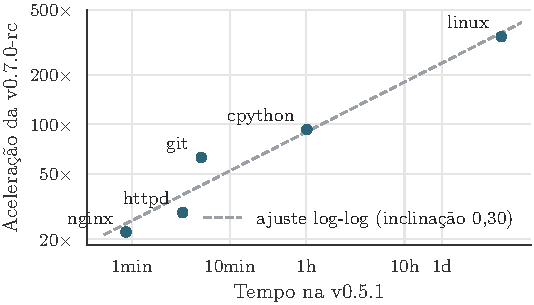
\includegraphics[width=0.8\linewidth]{figures/speedup_by_size.pdf}
\caption{Aceleração por repositório em função do tempo na \texttt{v0.5.1}. A reta tracejada é o ajuste em log-log.}
\label{fig:speedup}
\end{figure}

Reduzir a similaridade de 1,00 para 0,80 na \vnova{} aumentou o tempo em todos os repositórios (Tabela~\ref{tab:sim}), com efeito maior nos projetos maiores, e aumentou o tamanho do cache em 16,4\%.

\begin{table}[ht!]
\centering
\caption{Variação do tempo na \vnova{} ao passar da similaridade 1,00 para 0,80.}
\label{tab:sim}
\begin{tabular}{lrr}
\toprule
\textbf{Repositório} & \textbf{Tempo com 1,00} & \textbf{Variação com 0,80} \\
\midrule
Linux & 16 min 57 s & +2.237\% \\
\textsc{CPython} & 39 s & +563\% \\
llvm-project & 28 min 59 s & +307\% \\
\textsc{Git} & 4,9 s & +133\% \\
\textsc{NGINX} & 2,4 s & +100\% \\
httpd & 6,8 s & +93\% \\
\bottomrule
\end{tabular}
\end{table}

A Figura~\ref{fig:simheat} mostra a mesma comparação por repositório: a coluna de referência traz o tempo absoluto e as demais, a variação em relação a ela.

Na \texttt{v0.5.1}, o limiar não deveria afetar o tempo de forma sistemática, pois o cálculo de similaridade não era interrompido antecipadamente (a terminação antecipada só aparece na \texttt{v0.6.0}); no Linux e no \textsc{CPython}, a variação foi de $+2\%$ e $-3\%$. As reduções de $37\%$ a $58\%$ no \textsc{NGINX}, no httpd e no \textsc{Git} com 0,80 são, portanto, mais compatíveis com variação entre execuções do que com efeito do limiar: cada configuração foi executada uma única vez, em máquina virtual, sem medida de variância.

\begin{figure}[ht!]
\centering
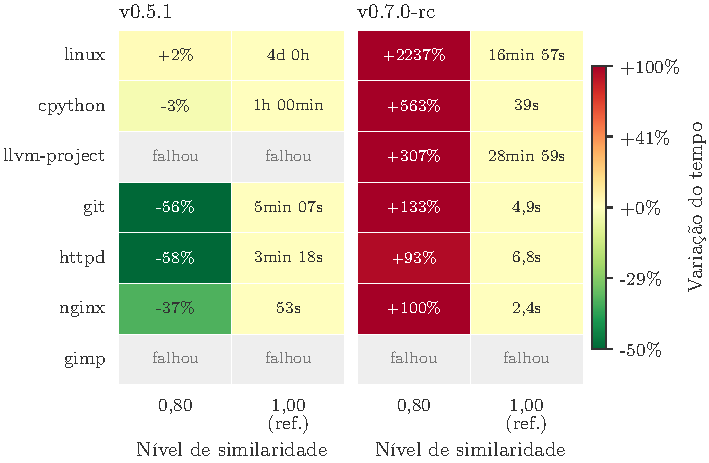
\includegraphics[width=\linewidth]{figures/similarity_heatmap.pdf}
\caption{Variação do tempo de execução por repositório e nível de similaridade. A escala de cores satura em metade e no dobro do tempo da referência.}
\label{fig:simheat}
\end{figure}

\subsection{Visualizações de duplicação}\label{sec:viz}

\scene{Scene 4v}{6:30--7:10}

As Figuras~\ref{fig:treemap} e~\ref{fig:hebundling} mostram as duas visualizações aplicadas ao kernel Linux. Elas respondem a perguntas diferentes: os feixes mostram \emph{entre quais partes} do projeto a duplicação acontece, e o mapa de árvore mostra \emph{quanto} código duplicado existe e \emph{onde}.

\begin{figure}[htbp]
    \centering
    \begin{subfigure}[t]{0.48\textwidth}
        \centering
        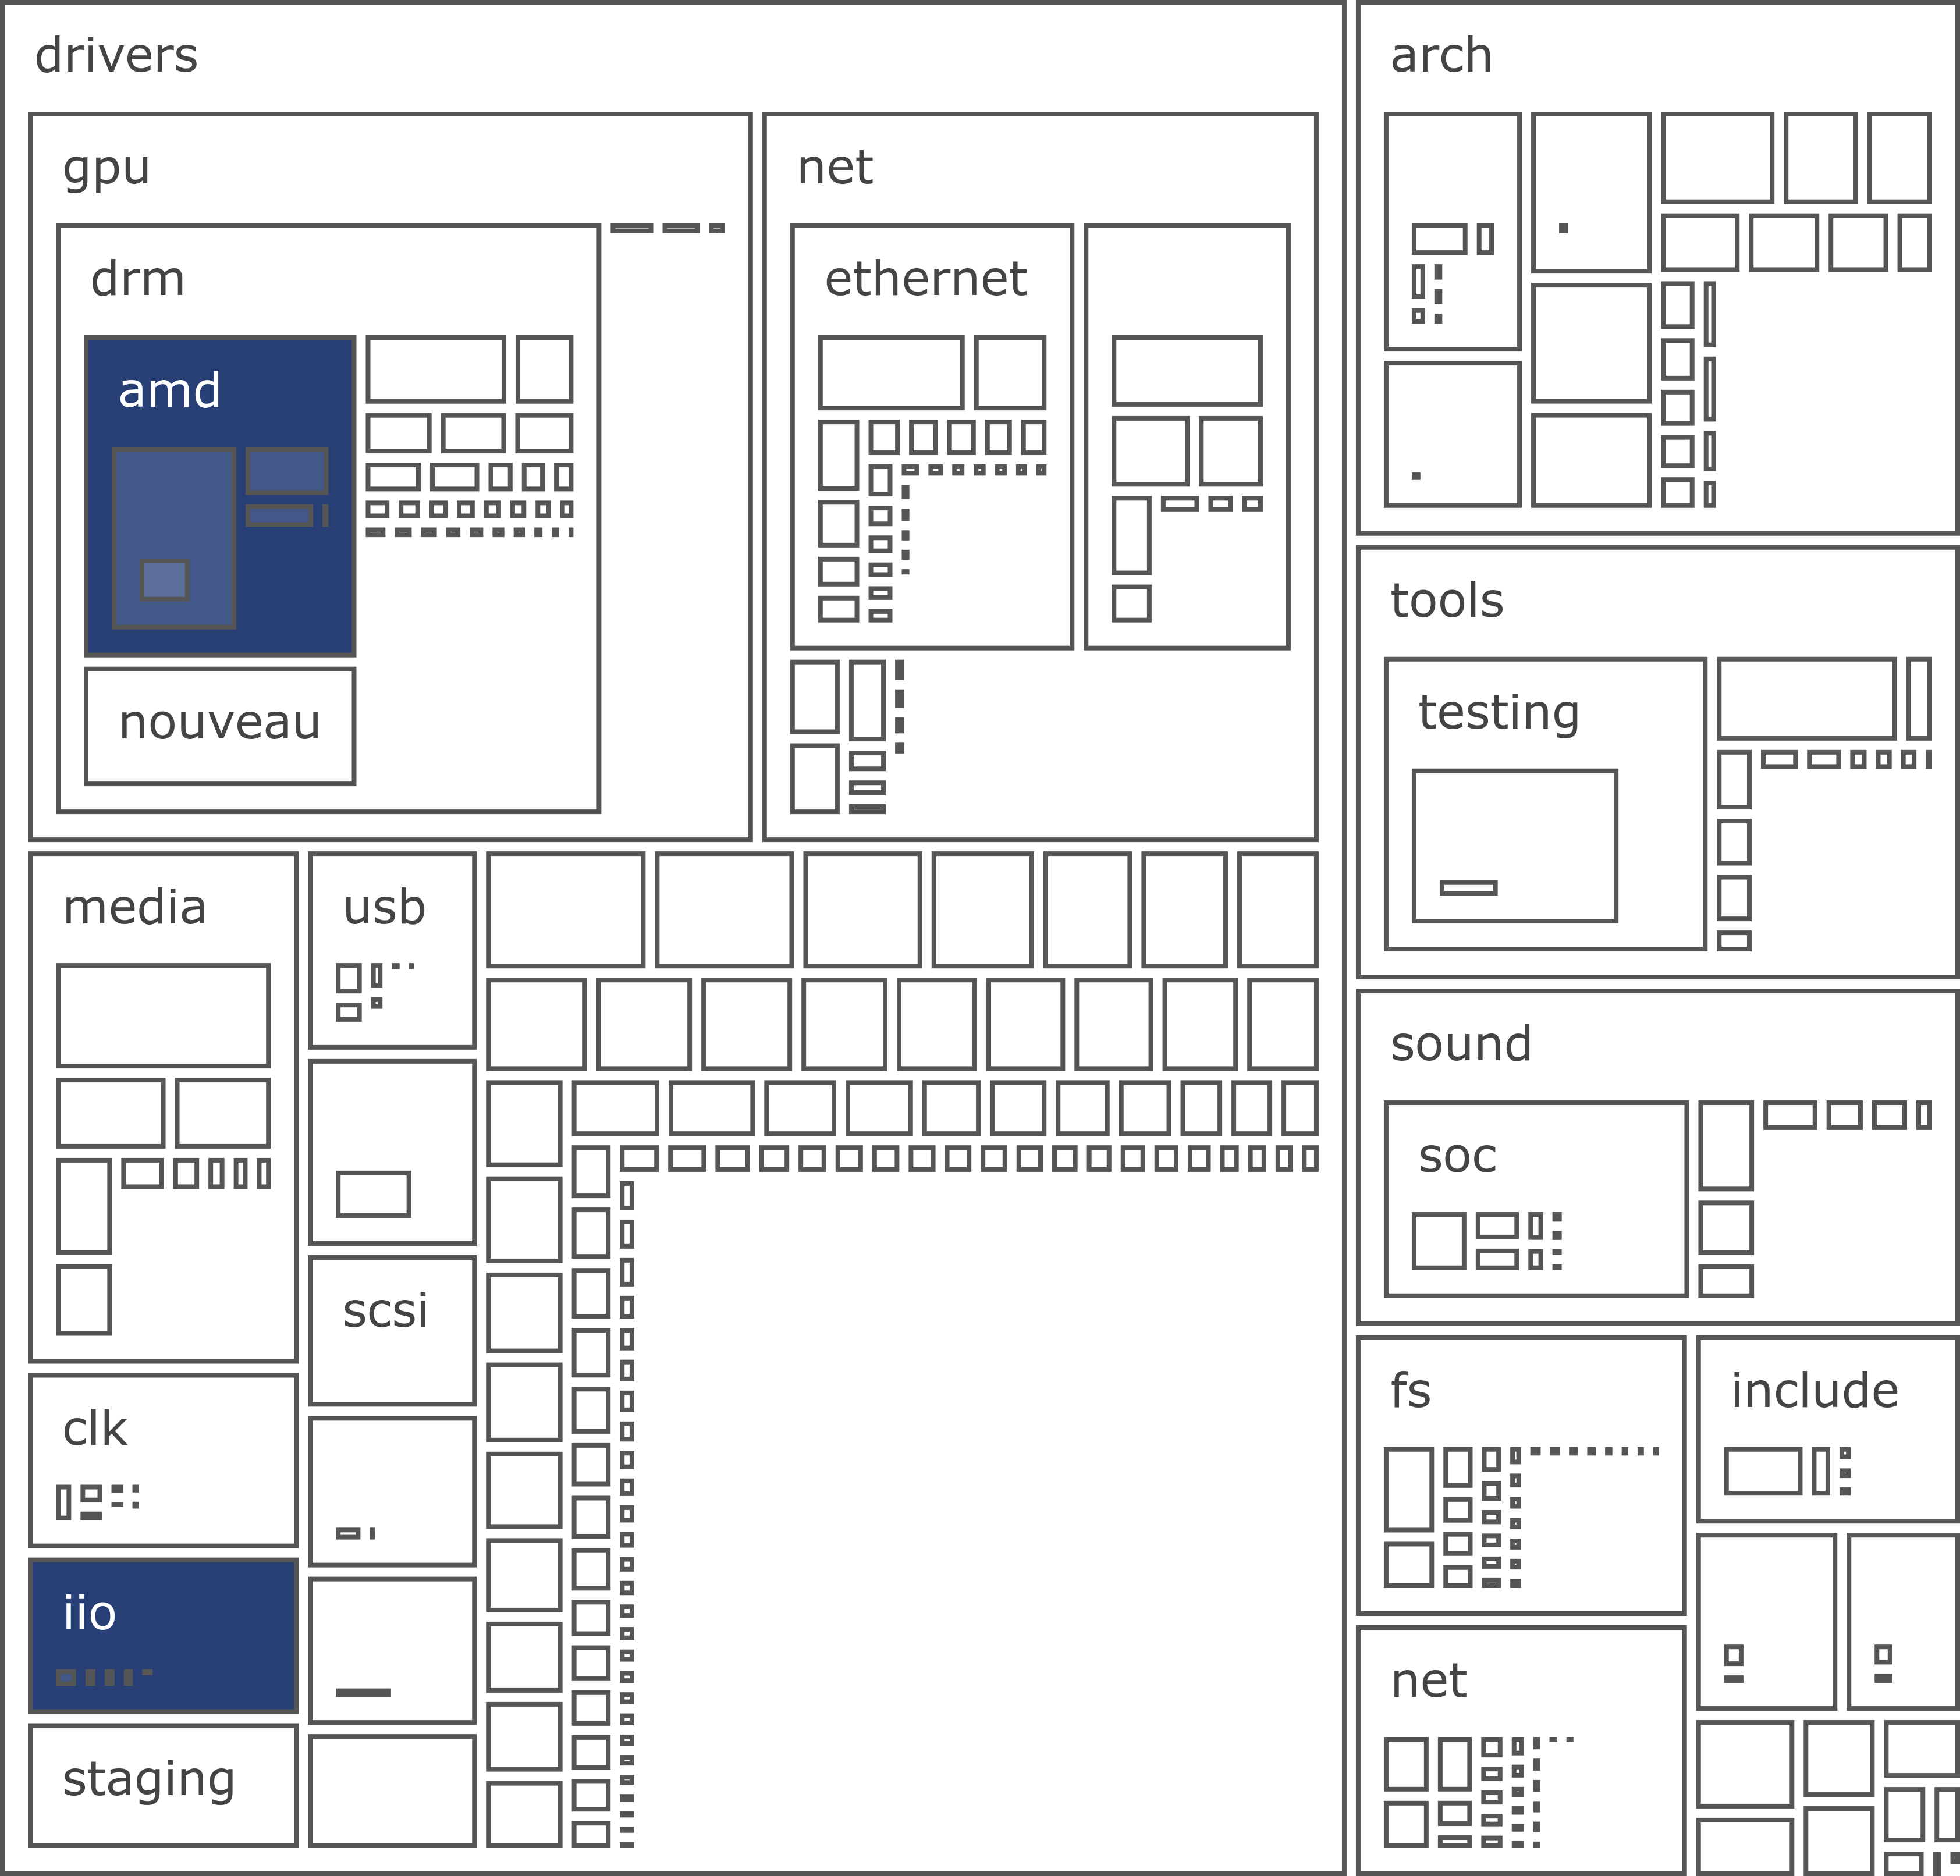
\includegraphics[width=\textwidth]{figures/treemap-linux.png}
        \caption{Mapa de árvore da duplicação no kernel Linux. A área de cada arquivo é proporcional à similaridade ponderada $\mathrm{WS}(p)$; os retângulos externos são diretórios.}
        \label{fig:treemap}
    \end{subfigure}
    \hfill
    \begin{subfigure}[t]{0.48\textwidth}
        \centering
        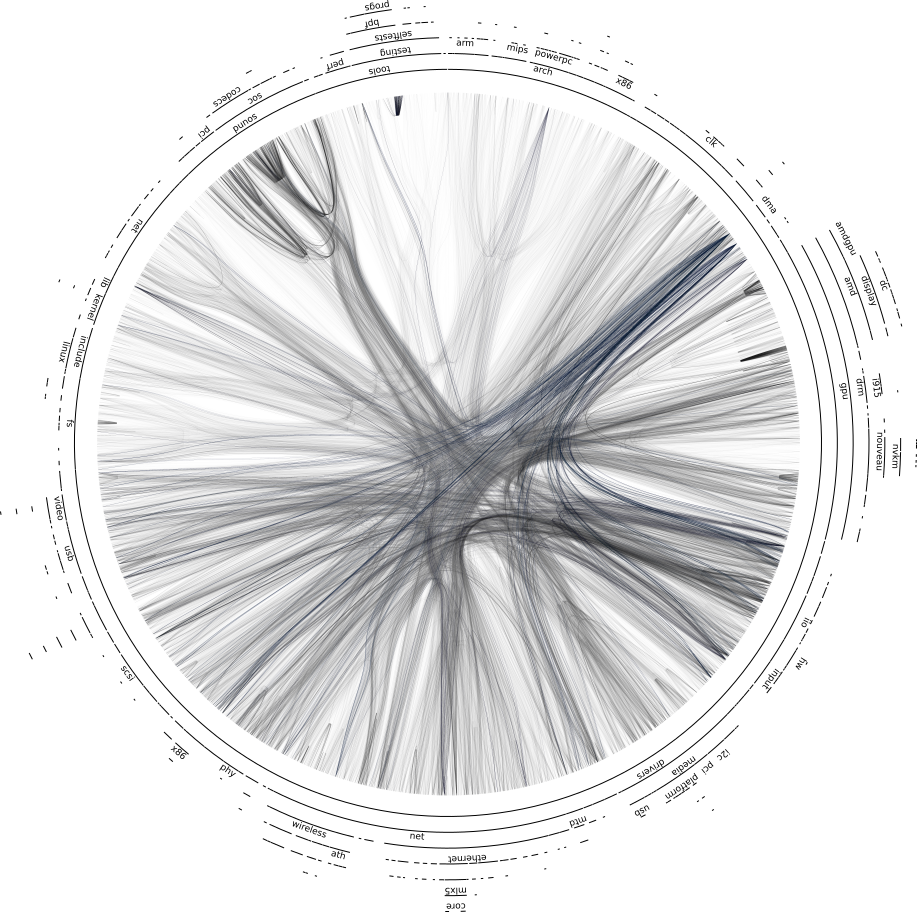
\includegraphics[width=\textwidth]{figures/edge-bundling-linux.png}
        \caption{Feixes hierárquicos de arestas da duplicação entre arquivos do kernel Linux. Os anéis externos indicam a hierarquia de diretórios (\texttt{arch}, \texttt{drivers}, \texttt{net}, \texttt{sound}, \texttt{tools} etc.).}
        \label{fig:hebundling}
    \end{subfigure}
\end{figure}

No mapa de árvore, \texttt{drivers} ocupa a maior parte da área, com \texttt{drivers/\allowbreak gpu/\allowbreak drm/\allowbreak amd} entre os maiores blocos, seguido de \texttt{arch}, \texttt{sound}, \texttt{net} e \texttt{tools}. Os subsistemas AMDGPU e IIO (\texttt{drivers/iio}), alvos do projeto de iniciação científica, aparecem destacados.

\paragraph{Trabalho futuro: matriz de dispersão de clones.} Uma terceira visualização segue a matriz usada por Yu e Ramaswamy~\cite{yu2008clones} para o Linux 2.4.20: os arquivos são ordenados pelo caminho nos dois eixos, cada par de clones vira um ponto e os diretórios aparecem como quadrados ao longo da diagonal. Pontos dentro de um quadrado são clones no mesmo diretório; pontos fora da diagonal são clones entre diretórios. Repetir a figura com o \ark{} na versão atual do kernel permite comparar a distribuição da duplicação com a observada em 2008.

\iffalse
\begin{figure}[ht!]
\centering
\missingfigure{Matriz de dispersão de clones do kernel Linux atual, no formato de Yu e Ramaswamy~\cite{yu2008clones}.}
\caption{Matriz de dispersão de clones.}
\label{fig:dotplot}
\end{figure}
\fi

\paragraph{Trabalho futuro: \textit{Hierarchical Edge Bundling} em 3D.} Lambert, Bourqui e Auber~\cite{lambert2010bundling3d} aplicaram o agrupamento de arestas a grafos sobre um globo e desenharam os feixes como tubos sombreados, o que facilita distinguir feixes que se cruzam. A proposta é levar a visualização da Figura~\ref{fig:hebundling} para uma esfera, com cada subsistema ocupando uma região e os feixes desenhados em 3D na renderização WebGL2 já existente. Com o kernel, a versão circular sobrepõe muitos feixes no centro do círculo; distribuir os arquivos sobre uma superfície deve reduzir essa sobreposição e permitir girar e aproximar regiões específicas.

\subsection{Análises em andamento}\label{sec:andamento}

As análises abaixo ficam como propostas para complementar os resultados de desempenho e robustez.

\paragraph{A1. Quantas funções colidem no cache.}
A \textit{issue} de colisão descreve o mecanismo, mas não o tamanho do problema. Basta contar, em cada projeto, quantos pares (arquivo, nome da função) aparecem mais de uma vez entre as funções extraídas pelo Tree-sitter, separando por causa (\texttt{\#ifdef}, sobrecarga em \cpp, métodos com mesmos nomes). Com o novo registro de funções, essa contagem pode ser feita no próprio ponto em que os identificadores são gerados.

\paragraph{A2. Efeito isolado da terminação antecipada.}
Rodar a \texttt{v0.5.4} e a \texttt{v0.6.0}, que diferem principalmente pela terminação antecipada, nos mesmos repositórios e limiares, e comparar os perfis do \texttt{perf} das duas. A diferença de tempo entre elas isola o ganho dessa otimização do restante das mudanças da \vnova{}.

\paragraph{A3. Normalização por tamanho e complexidade empírica.}
Medir o número de linhas de código com o \texttt{cloc} e o número de funções no cache de cada projeto. Com isso: (i) pares por mil linhas, que permitem comparar projetos; (ii) tempo contra número de funções em log-log por versão, cuja inclinação estima a complexidade e explica a aceleração crescente da Figura~\ref{fig:speedup}.

\subsection{Possíveis contribuições identificadas}\label{sec:possiveis}

\scene{Scene 4d}{7:10--7:45}

A triagem preliminar (Seção~\ref{sec:triagem}) produziu uma lista de casos que podem virar contribuições. Eles não são apresentados como resultado: são hipóteses a confirmar manualmente. A Tabela~\ref{tab:possiveis} lista os casos, nos projetos analisados, que a triagem apontou como mais promissores, cada um com o indício encontrado no histórico.

{\small\setlength{\tabcolsep}{4pt}
\begin{longtable}{P{0.15\linewidth}P{0.40\linewidth}P{0.37\linewidth}}
\caption{Possíveis contribuições de refatoração apontadas pela análise preliminar.}
\label{tab:possiveis}\\
\toprule
\textbf{Projeto} & \textbf{Duplicação} & \textbf{Indício a confirmar} \\
\midrule
\endfirsthead
\toprule
\textbf{Projeto} & \textbf{Duplicação} & \textbf{Indício a confirmar} \\
\midrule
\endhead
\bottomrule
\endlastfoot
\textsc{CPython} & \texttt{\_curses\_window\_\allowbreak addnstr\_impl} e \texttt{\_insnstr\_impl} & Correção de vazamento aplicada a três funções em \texttt{8060aa5d7dd} e à quarta só em \texttt{23180c50082}. \\
httpd & \texttt{handle\_headers} em \texttt{mod\_authnz\_fcgi} e \texttt{mod\_proxy\_fcgi} & Correção do CVE-2014-3583\footnote{\url{https://www.cve.org/CVERecord?id=CVE-2014-3583}} aplicada às duas cópias em \texttt{54f079749858}. \\
httpd & \texttt{include\_cgi} em \texttt{mod\_cgi} e \texttt{mod\_cgid} & O projeto já move funções comuns para \texttt{cgi\_common.h} (\texttt{eabfcda175c1}). \\
\textsc{NGINX} & \texttt{ngx\_http\_proxy\_\allowbreak set\_ssl} e \texttt{ngx\_http\_uwsgi\_\allowbreak set\_ssl} & Correções de TLS aplicadas às duas cópias (ex.: \texttt{fe43346dc315}). \\
\textsc{NGINX} & \texttt{ngx\_http\_scgi\_\allowbreak process\_header} e \texttt{ngx\_http\_uwsgi\_\allowbreak process\_header} & Correções de \emph{parsing} de cabeçalhos nas duas cópias. \\
\textsc{NGINX} & Cliente HTTP/2 em \texttt{ngx\_http\_grpc\_module.c} e \texttt{ngx\_http\_proxy\_v2\_module.c} & Arquivo recente copiado do módulo gRPC e alterado em conjunto depois. \\
\end{longtable}}

A análise também sugeriu possíveis \textit{issues} para o próprio \ark{}, ainda não reproduzidas: macros em caixa-alta, como \texttt{LIBC\_NAMESPACE\_DECL} no \textsc{LLVM}, interpretadas como funções; funções reportadas com linha inicial 0 em \textit{fixtures} de teste do \textsc{Git}; e pares de tamanhos muito diferentes reportados com similaridade 1,0. Se confirmados, cada um vira uma \textit{issue} para a ferramenta. A análise indicou ainda que boa parte da duplicação nos projetos é intencional (subsistemas paralelos, código gerado, de terceiros ou de teste), o que é coerente com os cenários de tolerância à duplicação observados pelo grupo no kernel Linux~\cite{duplicationdebt2026}.

\section{Discussão}

\scene{Scene 5}{7:45--9:30}

\paragraph{Projetos reais como teste da ferramenta.}
Os problemas mais graves surgiram de entradas que dificilmente fariam parte de uma suíte de testes da ferramenta: um arquivo de teste do \textsc{LLVM} construído para quebrar \emph{parsers} e funções com mesmos nomes separadas por diretivas de pré-processador. Os dois afetam tipos diferentes de qualidade. O \emph{stack overflow} interrompe a análise inteira de um repositório de quase 600 mil \textit{commits} por causa de um único arquivo; a colisão de cache produz falsos negativos silenciosos e resultados que dependem da ordem de leitura.

\paragraph{Desempenho depende do tamanho de entrada.}
A aceleração da \vnova{} vai de 22 vezes no \textsc{NGINX} a 342 vezes no Linux. Como a terminação antecipada economiza mais quanto mais pares diferentes houver, o ganho só aparece por inteiro em bases grandes, e teria sido subestimado se a ferramenta fosse avaliada apenas em repositórios pequenos. O limiar escolhido pelo usuário passa a ter um custo visível: com 0,80, o tempo aumenta 93\% no httpd e 2.237\% no Linux.

\paragraph{Manter a ferramenta para usá-la em escala.}
Boa parte do trabalho no período não foi de detecção de clones, mas de manutenção: integração contínua, avisos de compilação, atualização de dependências, portabilidade e documentação. Esse trabalho reduz o custo de reproduzir as execuções em outras máquinas e de receber contribuições externas.

\paragraph{Visualizar antes de selecionar.}
Com milhões de pares, listas e tabelas não mostram onde a duplicação se concentra. As visualizações trocam a unidade de análise da função para o arquivo e o diretório, e permitem escolher onde olhar primeiro antes da análise detalhada. Os feixes de arestas mostram relações entre partes do projeto; o mapa de árvore mostra volume. As duas perdem o detalhe de quais funções estão envolvidas, que continua dependendo da saída da ferramenta.

\paragraph{De duplicação detectada a contribuição.}
A ferramenta encontra muitos pares em bases grandes, e transformar essa saída em contribuições exige outro tipo de trabalho: separar código gerado, de terceiros e de teste, entender se a duplicação é intencional e procurar no histórico evidência de que ela já custou algo.

\paragraph{Limitações.}
Cada configuração de execução rodou uma única vez, em uma máquina virtual, sem medida de variância, o que limita a interpretação de diferenças pequenas e das variações da \texttt{v0.5.1} entre limiares (Figura~\ref{fig:simheat}). A comparação entre \texttt{v0.5.1} e \vnova{} mistura várias mudanças, e o efeito de cada uma não foi isolado. A análise de possíveis contribuições não foi verificada integralmente.

\section{Conclusão}

\scene{Scene 6}{9:30--10:15}

Executar o \ark{} em sete projetos FLOSS de grande porte revelou problemas da ferramenta: um \emph{crash} por recursão profunda, colisões de cache entre funções com mesmos nomes e falhas na extração de nomes em \cpp, além de necessidades de uso em bases grandes. Esses achados viraram \textit{issues} e correções. No período foram publicadas cinco versões da ferramenta, com a terminação antecipada no cálculo de similaridade, guiada por perfis de execução, um novo armazenamento binário, além de duas visualizações da duplicação no kernel Linux. Entre a \texttt{v0.5.1} e a \vnova{}, a taxa de sucesso subiu de 71\% para 86\% e o kernel Linux passou de cerca de 4 dias para menos de 17 minutos de análise, com uma aceleração que cresce com o tamanho do projeto. As execuções também produziram uma lista de possíveis contribuições aos projetos analisados, que está em verificação.

\subsection{Próximos passos}

\scene{Scene 7}{10:15--11:00}

\begin{itemize}
  \item Incluir a assinatura ou a posição da função na identidade usada no cache.
  \item Concluir a integração do armazenamento binário e lançar a \texttt{v0.7.0}.
  \item Confirmar manualmente os casos da Tabela~\ref{tab:possiveis} e as possíveis \textit{issues} da ferramenta, e submeter os que se confirmarem.
  \item Concluir a matriz de dispersão de clones, gerar as visualizações para os demais projetos analisados e implementar os feixes de arestas em 3D.
  \item Investigar a falha no \textsc{GIMP}.
  \item Implementar as opções \texttt{-{}-exclude} e de metadados do repositório propostas nas \textit{issues}.
\end{itemize}

\section*{Disponibilidade dos artefatos}\label{sec:artefatos}

Os artefatos deste trabalho estão em um repositório público: \url{https://github.com/guilhermeivo/research-linux-kernel-duplications}. Incluindo o código \LaTeX{} deste relatório e as figuras; os \textit{scripts} de execução e de análise (tempo, taxa de sucesso, tamanho do \textit{cache}, mapa de calor e ajuste log-log).

\clearpage

\bibliographystyle{abnt}
\bibliography{references}

\clearpage
\appendix

\section{Histórico de Atividades}\label{sec:historico}

A tabela a seguir apresenta a distribuição das 100 horas de atividades consideradas para fins de integralização da disciplina, realizadas entre agosto e novembro de 2026. As atividades de desenvolvimento podem ser conferidas no histórico de commits e de \emph{merge requests} do repositório do \ark{}.

\begin{longtable}{P{2.1cm} P{8cm} r}
\caption{Histórico das atividades e horas dedicadas.}
\label{tab:historico}\\
\toprule
\textbf{Período} & \textbf{Atividade desenvolvida} & \textbf{Horas} \\
\midrule
\endfirsthead
\toprule
\textbf{Período} & \textbf{Atividade desenvolvida} & \textbf{Horas} \\
\midrule
\endhead
\midrule
\multicolumn{3}{r}{\footnotesize continua na próxima página}\\
\endfoot
\bottomrule
\endlastfoot
\multicolumn{3}{l}{\textit{Agosto -- seleção, ambiente e primeira execução}}\\
03/08--09/08 & Seleção dos projetos FLOSS (\textsc{NGINX}, \textsc{Git}, httpd, \textsc{CPython}, Linux, \textsc{LLVM}, \textsc{GIMP}) a partir de tamanho, linguagem e histórico. & 3 \\
10/08--27/08 & Configuração do ambiente: compilação do \ark{} \texttt{v0.5.1} com opções de depuração, clones completos dos 7 repositórios e scripts de execução em lote. & 4 \\
17/08--31/08 & Execução da \texttt{v0.5.1} nos 7 repositórios e levantamento inicial das falhas (\emph{crash} no \textsc{LLVM}, falha no \textsc{GIMP}, erros de \emph{parsing}). & 9 \\
24/08--28/08 & Correção da extração de nomes de funções \cpp{} no \emph{parser} e publicação da \texttt{v0.5.2}. & 3 \\
\midrule
\multicolumn{3}{l}{\textit{Setembro -- investigação, issues e integração contínua}}\\
01/09--15/09 & Reprodução do \emph{stack overflow} no \textsc{LLVM} com \textsc{GDB}, análise do \emph{backtrace} e identificação de \texttt{parser\_overflow.c}. & 5 \\
01/09--15/09 & Investigação de falsos negativos por funções homônimas (\texttt{apply\_acpi\_orientation} no Linux, sobrecarga \cpp, métodos homônimos). & 5 \\
16/09--30/09 & Investigação de resultados suspeitos nas saídas da ferramenta e conferência manual no código-fonte. & 3 \\
16/09--30/09 & Abertura da issue do \emph{stack overflow} e relato na discussão de execuções em projetos reais. & 3 \\
16/09--30/09 & Análise dos dados das execuções e gráficos: taxa de sucesso, tempos por repositório, efeito da similaridade, tamanho do cache. & 3 \\
16/09--08/10 & Visualizações de duplicação: feixes hierárquicos de arestas com renderização em WebGL2 e mapa de árvore ponderado por similaridade. & 11 \\
\midrule
\multicolumn{3}{l}{\textit{Outubro -- armazenamento, reexecução e análise}}\\
01/10--15/10 & Registro de funções com identificadores FNV-1a e migração do armazenamento das duplicações para formato binário; centralização do caminho de saída em \texttt{FunctionStorage} e publicação da \texttt{v0.5.3}. & 10 \\
01/10--15/10 & Execução da \vnova{} com similaridade 1,00 e 0,80 nos 7 repositórios; coleta de tempo, status e tamanho do cache. & 6 \\
16/10--31/10 & Análise comparativa das rodadas (tempo, falhas, cache, efeito da similaridade). & 5 \\
16/10--31/10 & Triagem preliminar das duplicações com scripts; verificação manual dos candidatos no código e no histórico do git. & 6 \\
16/10--31/10 & Desenvolvimento e testes locais de refatorações nos projetos analisados. & 8 \\
\midrule
\multicolumn{3}{l}{\textit{Novembro -- desempenho, manutenção e novas issues}}\\
01/11--12/11 & Análise de desempenho com \texttt{perf}, terminação antecipada no cálculo de similaridade entre árvores e publicação das versões \texttt{v0.5.4}, \texttt{v0.6.0} e \texttt{v0.6.1}. & 6 \\
12/11--20/11 & Avisos de compilação, reorganização do CMake, atualização da libgit2 e do PCRE2. & 7 \\
16/11--23/11 & Abertura das issues de metadados do repositório, exclusão de arquivos/diretórios e colisão de cache; atualização da discussão com o caso do Linux. & 3 \\
\midrule
\multicolumn{2}{r}{\textbf{Total}} & \textbf{100} \\
\end{longtable}
\normalsize

\end{document}
